\documentclass[tikz]{standalone}

\usepackage{tikz}
\usetikzlibrary{positioning}

\begin{document}

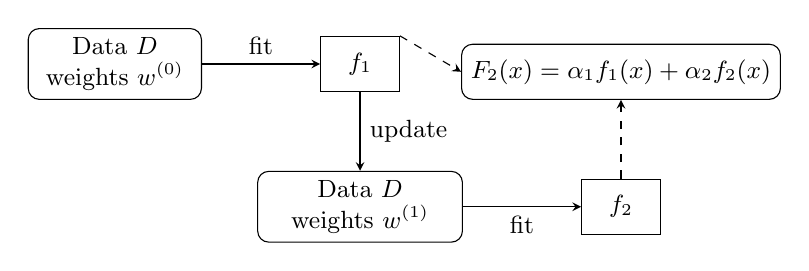
\begin{tikzpicture}[
    >=stealth,
    every node/.style={font=\small},
    box/.style={draw,rounded corners,minimum width=22mm,minimum height=7mm,align=center},
    tree/.style={draw,rectangle,minimum width=10mm,minimum height=7mm,align=center}
]

% Data with weights
\node[box] (d0) {Data $D$\\weights $w^{(0)}$};

% First tree
\node[tree,right=15mm of d0] (f1) {$f_1$};
\draw[->] (d0) -- node[above]{fit} (f1);

% Reweighted data
\node[box,below=10mm of f1,minimum width=26mm] (d1) {Data $D$\\weights $w^{(1)}$};
\draw[->] (f1.south) -- node[right]{update} (d1.north);

% Second tree
\node[tree,right=15mm of d1] (f2) {$f_2$};
\draw[->] (d1) -- node[below]{fit} (f2);

% Ensemble arrows
\node[box,above=10mm of f2,minimum width=30mm] (F) {$F_2(x)=\alpha_1 f_1(x)+\alpha_2 f_2(x)$};

\draw[->,dashed] (f1.north east) -- (F.west);
\draw[->,dashed] (f2.north)      -- (F.south);

\end{tikzpicture}

\end{document}

